% Spectrum of release models --- plan \S4.13 (Phase 4, FULL DETAIL by
% decision).
% Sources: new_notes3 Part F \S26--\S29 (skeleton + summaries);
% new_notes2 \S14 (Cases 1--5), \S12 (reset), \S15 (self-excitation),
% \S16 (partial release).
% Notation fixes vs the sources: eclipse conversion rate written \alpha
% (not a, which is a root); telegraph switching \sigma_{\rm on/off}
% (not \alpha/\lambda); eclipse division \rho_{\rm div} (not \rho).

\section{The spectrum of release models}
\label{sec:spectrum}

Bursting and constant budding are the two ends of a spectrum, and the
renewal construction of \S\ref{sec:renewal} is the bridge between them:
\emph{any} intracellular model that supplies a survival kernel $S(a)$ and a
release kernel $g(a)$ induces the same population skeleton. This section
lays out the spectrum. First the skeleton and the classical models built on
it (\S\ref{sec:skeleton}--\S\ref{sec:five-cases}); then reset catastrophe,
which interpolates by letting one cell release many times
(\S\ref{sec:reset}); then self-exciting release (\S\ref{sec:self-excite});
and finally partial release, which interpolates in \emph{how much} leaves
the cell at an event (\S\ref{sec:boolean}). The evolutionary comparison
between the ends of the spectrum was made in \S\ref{sec:flooding}; its
ecological context belongs to Chapter~6. The whole arrangement is sketched
in Figure~\ref{fig:spectrum-map};
Figure~\ref{fig:N4b_3_release_spectrum} gives the same mechanisms ordered
by their generation-time structure, with the multi-stage contrast class of
\S\ref{sec:hiv} attached.

\begin{figure}[H]
\centering
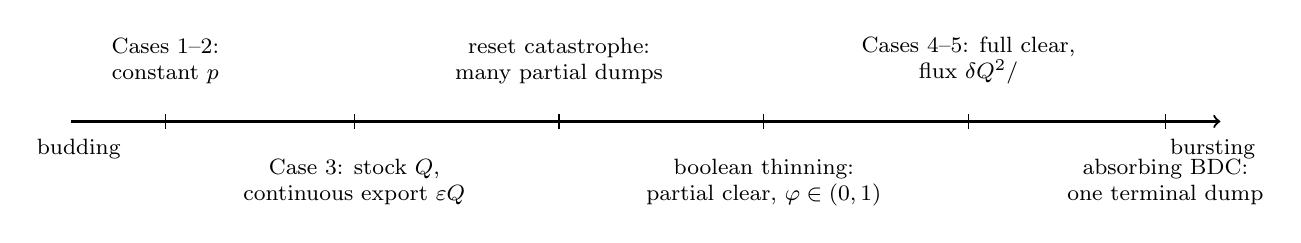
\begin{tikzpicture}
\draw[->,line width=0.8pt] (0,0) -- (14.6,0);
\node[below] at (0.1,-0.1) {\footnotesize budding};
\node[below] at (14.5,-0.1) {\footnotesize bursting};
\foreach \x/\lab/\side in {%
  1.2/{Cases 1--2:\\ constant $p$}/above,
  3.6/{Case 3: stock $Q$,\\ continuous export $\varepsilon Q$}/below,
  6.2/{reset catastrophe:\\ many partial dumps}/above,
  8.8/{boolean thinning:\\ partial clear, $\varphi\in(0,1)$}/below,
  11.4/{Cases 4--5: full clear,\\ flux $\delta Q^2/\Icell$}/above,
  13.9/{absorbing BDC:\\ one terminal dump}/below}
{\draw (\x,-0.09) -- (\x,0.09);
 \node[\side=0.35cm,align=center,font=\footnotesize] at (\x,0) {\lab};}
\end{tikzpicture}
\caption{The budding--bursting spectrum. Moving right, release becomes more
concentrated in time and more load-dependent: from constant budding (Cases
1--2) through stock-and-export (Case~3), recurrent partial dumps (reset
catastrophe), a tunable fraction $\varphi$ per event (boolean thinning),
load-proportional full clear (Cases 4--5), to the single terminal dump of
the absorbing BDC of this chapter.}
\label{fig:spectrum-map}
\end{figure}

\begin{figure}[H]
\centering
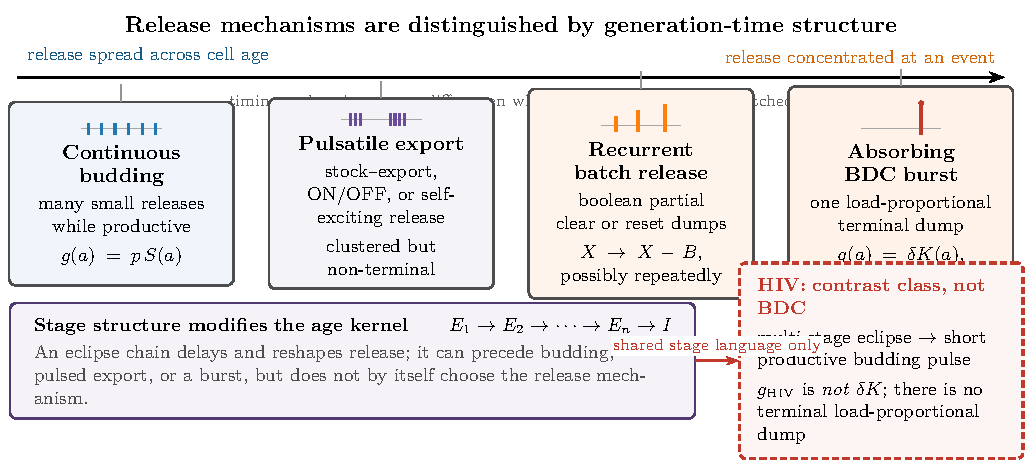
\includegraphics[width=0.95\textwidth]{figures/N4b_3_release_spectrum.pdf}
\caption{Spectrum of release mechanisms ordered by generation-time structure, from continuous production through pure bursting and modular variants. Multi-stage compartmental release models are shown as a contrast class, not as instances of the absorbing BDC process of this chapter.}
\label{fig:N4b_3_release_spectrum}
\end{figure}

\subsection{The universal renewal skeleton}
\label{sec:skeleton}

With incidence $i(t)=\gamma T\,\Vfree(t)$ (or a nonlinear incidence
$f(\Vfree,T)$), any choice of kernels gives
\begin{equation}
\Icell(t)=\Icell_0\,S(t)+(i*S)(t),
\qquad
\ddt{\Vfree}=\Icell_0\,g(t)+(i*g)(t)-c\,\Vfree(t),
\label{eq:skeleton}
\end{equation}
with effective parameters $p_{\rm eff}(r)=\Lap{g}(r)/\Lap{S}(r)$ and, for
linear incidence, $R_0=(\gamma T/c)\int_0^\infty g$. The models of this
section differ only in their $(S,g)$:
\begin{center}
\renewcommand{\arraystretch}{1.2}
\small
\begin{tabular}{@{}lll@{}}
\toprule
Model & $S(a)$ & $g(a)$ \\
\midrule
Classical BMVR & $e^{-d_{\Icell} a}$ & $p\,e^{-d_{\Icell} a}$ \\
Absorbing BDC (this chapter) & $\Ifix(a)$ & $\delta K(a)$ \\
MOI-$k$ BDC (Chapter~4a) & $I(a)^k-D(a)^k$ & $\delta K_k(a)$ \\
Reset catastrophe (\S\ref{sec:reset}) & $e^{-d_{\Icell} a}$ & $\delta e^{-d_{\Icell}a}\mean{X_a^2}$ \\
HIV multi-stage (\S\ref{sec:hiv}) & stage survival & $p\times$ productive occupancy \\
Two-type / GATE (Ch.~5) & two-type $\Ifix$ & two-type second-moment flux \\
\bottomrule
\end{tabular}
\end{center}
The first row is the check of Figure~\ref{fig:D-exp}: exponential kernels
reduce \eqref{eq:skeleton} exactly to classical BMVR.

\subsection{Five modular ODE cases}
\label{sec:five-cases}

When a finite-dimensional ODE description is wanted --- for fitting, or for
analytic tractability --- the same ideas assemble into a ladder of five
cases. Target cells $T$ are held fixed throughout; $\Icell$ denotes
productively infected cells, $\Vfree$ free particles, $E$ eclipse cells,
and $Q$ the total intracellular stock summed over infected cells. In all
five cases, production into the stock (once productive) is
\emph{mean-linear}, immigration-type, at rate $\nu$ per cell --- the choice
appropriate to template-limited intracellular accumulation
(\S\ref{sec:hiv-growth}); what distinguishes the cases is the release law
and the presence or absence of an eclipse class. In this subsection
$\alpha$ denotes the eclipse conversion rate; it is not the root $a$.

\subsubsection{Case 1 --- Classic BMVR}

An infected cell produces particles that are released immediately at
constant rate $p$ (budding). No eclipse, no stored pool; infected cells are
removed at rate $d_{\Icell}$:
\begin{equation}
\ddt{\Icell}=\gamma T\,\Vfree-d_{\Icell}\Icell,
\qquad
\ddt{\Vfree}=p\,\Icell-c\,\Vfree,
\qquad
R_0=\frac{\gamma T\,p}{c\,d_{\Icell}}.
\end{equation}
Production and export are collapsed into the single phenomenological
parameter $p$. This is the model the rest of the chapter is replacing.

\subsubsection{Case 2 --- Eclipse + classic release}

New infections enter an eclipse class $E$ --- infected but not yet
producing --- and convert to productive cells at rate $\alpha$ (mean
eclipse length $1/\alpha$), with optional eclipse death $d_E$:
\begin{equation}
\ddt{E}=\gamma T\,\Vfree-(\alpha+d_E)E,
\qquad
\ddt{\Icell}=\alpha E-d_{\Icell}\Icell,
\qquad
\ddt{\Vfree}=p\,\Icell-c\,\Vfree,
\end{equation}
\begin{equation}
R_0=\frac{\gamma T}{c}\cdot\frac{\alpha}{\alpha+d_E}\cdot\frac{p}{d_{\Icell}}.
\end{equation}
A fraction $\alpha/(\alpha+d_E)$ of eclipse cells become productive; each
then yields mean $p/d_{\Icell}$ particles. Setting $\alpha\to\infty$ with
$d_E=0$ recovers Case~1. A more realistic eclipse-time distribution is an
Erlang chain $E_1\to\cdots\to E_n\to\Icell$, each step at rate $\alpha$;
the $\Vfree$ equation is unchanged. This is the standard delay construction
of the within-host literature --- and, as \S\ref{sec:hiv} will emphasise,
it is inserted by hand there, whereas in the two-type BDC it emerges
mechanically (the GATE observation of Chapter~5).

\subsubsection{Case 3 --- Intracellular stock + continuous export}

Productively infected cells accumulate stock at rate $\nu$ per cell; each
intracellular unit is exported at per-capita rate $\varepsilon$; cell death
removes the cell and its share of stock:
\begin{equation}
\ddt{\Icell}=\gamma T\,\Vfree-d_{\Icell}\Icell,
\qquad
\ddt{Q}=\nu\Icell-\varepsilon Q-d_{\Icell}Q,
\qquad
\ddt{\Vfree}=\varepsilon Q-c\,\Vfree.
\end{equation}
The mean load per productive cell is $m=Q/\Icell$. In the quasi-steady
stock regime ($\ddt Q\approx0$),
\begin{equation}
Q_*=\frac{\nu}{\varepsilon+d_{\Icell}}\,\Icell,
\qquad
p_{\mathrm{eff}}:=\frac{\varepsilon Q_*}{\Icell}
=\frac{\varepsilon\nu}{\varepsilon+d_{\Icell}},
\end{equation}
and Case~3 collapses to Case~1 with $p=p_{\mathrm{eff}}$: \emph{classical
BMVR is the fast-export limit of stock-and-export dynamics}. When export is
not fast, $\Vfree$ lags and depends on the history of $Q$. With eclipse
stacked in front (incidence into $E$, conversion at $\alpha$, only $\Icell$
producing), the $Q$ and $\Vfree$ equations are unchanged and eclipse cells
contribute nothing until conversion. The reproduction number is
\begin{equation}
R_0=\frac{\gamma T\,\nu\,\varepsilon}{c\,d_{\Icell}(\varepsilon+d_{\Icell})}
\qquad\text{(no eclipse)},
\end{equation}
which is Case~1's $R_0$ with $p=\varepsilon\nu/(\varepsilon+d_{\Icell})$.

\subsubsection{Case 4 --- Intracellular stock + proportional full clear}

The same accumulation, but release now comes in load-proportional dumps: in
a cell with load $x$, dumps occur at rate $\delta x$ and the whole pool is
transferred (the cell survives the dump; death remains the separate rate
$d_{\Icell}$). Under the homogeneous-load closure $x\approx m=Q/\Icell$,
the population dump flux is $\delta\,\mean{\sum_i X_i^2}\approx
\delta\Icell m^2=\delta Q^2/\Icell$, giving
\begin{equation}
\ddt{\Icell}=\gamma T\,\Vfree-d_{\Icell}\Icell,
\qquad
\ddt{Q}=\nu\Icell-\delta\frac{Q^2}{\Icell}-d_{\Icell}Q,
\qquad
\ddt{\Vfree}=\delta\frac{Q^2}{\Icell}-c\,\Vfree,
\end{equation}
with the convention that the nonlinear terms vanish when $\Icell=0$. The
dump term is simultaneously export into $\Vfree$ and clearance of $Q$; it
is quadratic in total load at fixed $\Icell$, i.e.\ superlinear in mean
load --- the mean-field echo of the superlinearity of $g_k$ in
Chapter~4a (\eqref{eq:gk}). The mature quasi-steady balance,
$\nu=\delta m^2+d_{\Icell}m$, gives
\begin{equation}
m=\frac{-d_{\Icell}+\sqrt{d_{\Icell}^2+4\delta\nu}}{2\delta},
\qquad
p_{\mathrm{eff}}=\delta m^2,
\end{equation}
which plays the role of $p$ only in that steady regime: transients and
early infection need the full $(Q,\Vfree)$ system. For invasion analysis
near $\Icell=0$, the map $Q\mapsto Q^2/\Icell$ is singular; one should
linearise the underlying single-cell process instead, taking
$R_0=\gamma T V_\infty/c$ as in the renewal framework.

\subsubsection{Case 5 --- Eclipse + stock + proportional full clear}

Case~2's eclipse block in front of Case~4: incidence creates eclipse cells;
only productive cells accumulate stock and dump:
\begin{equation}
\ddt{E}=\gamma T\,\Vfree-(\alpha+d_E)E,
\qquad
\ddt{\Icell}=\alpha E-d_{\Icell}\Icell,
\end{equation}
\begin{equation}
\ddt{Q}=\nu\Icell-\delta\frac{Q^2}{\Icell}-d_{\Icell}Q,
\qquad
\ddt{\Vfree}=\delta\frac{Q^2}{\Icell}-c\,\Vfree.
\end{equation}
Eclipse adds a further staged lag --- $E$ rises first, then $\Icell$ and
$Q$, then $\Vfree$ --- which Case~4 cannot produce; the quasi-steady
relations for the mean load among productive cells are unchanged. In the
single-cell sense,
\begin{equation}
R_0=\frac{\gamma T}{c}\cdot\frac{\alpha}{\alpha+d_E}\cdot V_\infty.
\end{equation}

\subsubsection{Summary of the five cases}

\begin{center}
\renewcommand{\arraystretch}{1.25}
\small
\begin{tabular}{@{}p{0.30\textwidth}p{0.34\textwidth}p{0.22\textwidth}@{}}
\toprule
Case & Intracellular story & Free-particle source term \\
\midrule
1 Classic & none (instant release) & $p\,\Icell$ \\
2 Eclipse + classic & delay $E\to\Icell$, then as 1 & $p\,\Icell$ \\
3 Stock + continuous export & $\nu$ into $Q$, export $\varepsilon Q$ & $\varepsilon\,Q$ \\
4 Stock + full clear & $\nu$ into $Q$, dump $\propto Q^2/\Icell$ & $\delta Q^2/\Icell$ \\
5 Eclipse + stock + full clear & $E\to\Icell$, then as 4 & $\delta Q^2/\Icell$ \\
\bottomrule
\end{tabular}
\end{center}
What is fixed across Cases~3--5 is the mean-linear production; what is
chosen is the release law and the presence of eclipse, and Case~5 is
exactly Case~4 composed with Case~2's eclipse block. Each case also induces
kernels $(S,g)$, so the convolution form \eqref{eq:skeleton} remains
available whenever the ODE stage structure is replaced by age structure ---
which is precisely the absorbing BDC at the bursting end of the ladder.

\subsection{Reset catastrophe}
\label{sec:reset}

The absorbing BDC releases at most once per cell. An intermediate worth
isolating lets a cell release \emph{many} times: while the cell is alive,
the load undergoes birth $\lambda n$, death $\mu n$, optional immigration
$\nu$, and a \emph{dump that resets}: at rate $\delta n$ the whole pool $n$
is released and the load returns to $0$, after which it may re-accumulate.
The cell itself dies at a separate rate $d_{\Icell}$, independent of the
load. Biologically, read the load as a local assembled pool rather than the
whole-cell contents: full dumping is one mathematical extreme of batch
release, budding is many small exports, and this process is a tractable
multi-pulse caricature between them.

Because dumps do not absorb, the kernels change but the skeleton does not:
\begin{equation}
S(a)=e^{-d_{\Icell}a},
\qquad
g(a)=\delta\,e^{-d_{\Icell}a}\,\mean{X_a^2},
\end{equation}
where $\mean{X_a^2}$ is computed for the non-absorbing reset process.
Linear rates keep the moments of that process tractable (closed ODEs under
the generator), so $g$ is explicit once they are solved; structurally,
$g\propto\mean{X^2}$ exactly as for the absorbing BDC. The renewal BMVR is
identical in form to \eqref{eq:Icell}--\eqref{eq:Vfree}, with
\begin{equation}
p_{\rm eff}(r)=\lrb{r+d_{\Icell}}\Lap{g}(r),
\qquad
d_{\Icell,{\rm eff}}\equiv d_{\Icell},
\end{equation}
and $R_0=(\gamma T/c)\int_0^\infty g$ --- finite only for $d_{\Icell}>0$,
since otherwise recurrent dumps could continue forever. If the reset process
admits a stationary law $\pi$ and $d_{\Icell}$ is small, the mature-cell
limit is
\begin{equation}
p_\infty=\lim_{a\to\infty}\frac{g(a)}{S(a)}=\delta\,\mean_\pi[X^2]:
\end{equation}
a long-lived infected cell behaves as classical constant-$p$ BMVR with that
$p$, while transients (first dumps, young cells) still need the full kernel.
An eclipse is added exactly as before: set $g(a)=0$ for $a<\tau_e$ and keep
$S(a)=e^{-d_{\Icell}a}$.

\begin{center}
\renewcommand{\arraystretch}{1.2}
\small
\begin{tabular}{@{}lll@{}}
\toprule
 & Absorbing BDC & Reset catastrophe \\
\midrule
After dump & process ends in $H$ & $X\to0$, continues \\
Dumps per cell & $\le1$ & many, until cell death \\
Survival kernel & $\Ifix$ & $e^{-d_{\Icell}a}$ \\
Release kernel & $\delta K_{\rm BDC}(a)$ & $\delta e^{-d_{\Icell}a}\mean{X_a^2}$ \\
Population equations & renewal BMVR & same form \\
Mature limit & not constant budding & $p\to\delta\mean_\pi[X^2]$ \\
\bottomrule
\end{tabular}
\end{center}

\subsection{Self-exciting release}
\label{sec:self-excite}

A further biological possibility is that release is partially
\emph{self-exciting}: one event makes further release more likely for a
short time --- cooperative nucleation, local membrane platforms, ESCRT
machinery already recruited at a site. The possibility must be balanced
against depletion of stock and finite machinery: pure open-ended
self-excitation is implausible, and a hybrid of excitation, refill and
depletion is the reasonable picture. Two levels of model are available, as
throughout: a renewal BMVR exists whenever the single-cell model defines
$(S,g)$; a finite ODE BMVR needs the excitation carried by a
low-dimensional Markov state.

The menu of candidates:
\begin{center}
\renewcommand{\arraystretch}{1.15}
\small
\begin{tabular}{@{}clp{0.26\textwidth}cc@{}}
\toprule
\# & Model & Excitation carried by & ODE BMVR? & Renewal? \\
\midrule
1 & Classical Hawkes & event history only & poor & yes (numerical $g$) \\
2 & Hawkes + stock $X$ & events + depletion/refill & via Model 10 & yes \\
3 & Marked Hawkes & size-weighted events & approximate & yes (numerical) \\
4 & ETAS-style & size + time kernel & approximate & yes (numerical) \\
5 & Cox + latent $Z$ & latent excitability & if $Z$ simple & yes \\
6 & ON/OFF telegraph & sustained high phase & yes & yes \\
7 & $\lambda\propto X^2$ & current load only & yes (Cases 4--5) & yes \\
8 & Nucleation biophysics & assembly cascade & hard & yes (numerical) \\
9 & Age since last release & renewal excitation & yes (stages) & yes \\
10 & Jumping rate $r(t)$ & shot-noise intensity & yes (mean-field) & yes \\
11 & Spatial Hawkes & local membrane & average first & after coarse-graining \\
12 & Full clear (Cases 4--5) & instant total cascade & yes & yes \\
\bottomrule
\end{tabular}
\end{center}
They nest: Model~2, with intensity $\lambda(t)=f(X_t)+\sum_{t_i<t}h(t-t_i)$,
is the general event-history form --- $h\equiv0$ and $f(x)=\varepsilon x$
recovers continuous export (Case~3); $h\equiv0$, $f(x)=\delta x^2$ with
full clear recovers Model~7 and Cases~4--5; an exponential
$h(t)=\eta e^{-\zeta t}$ is equivalent to Model~10; Model~6 is a coarse
two-level version without a continuous intensity. The four focal models:

\paragraph{Model 7 --- cooperative intensity, $\lambda(x)=\delta x^2$
(or $\delta x(x-1)$).} No memory of past events, only the current load:
more material makes release disproportionately more likely. The single-cell
process is production $\nu$, optional degradation $\mu X$, and full-clear
dumps at rate $\delta X^2$; the ODE form is exactly Cases~4--5 under the
homogeneous closure, and the renewal form has
$g(a)=\delta\,\mean{X_a^2\mathbf1\{\text{alive}\}}$. Cooperativity without
history; the default bulk ``excitatory'' model.

\paragraph{Model 6 --- ON/OFF telegraph.} The cell (or a membrane site)
switches between OFF and ON at rates $\sigma_{\rm on}$, $\sigma_{\rm off}$;
while ON it releases at rate $\rho$ (or $\varepsilon X$). Sample paths are
intermittent surges without full clear. The simplest ODE version splits the
infected class:
\begin{equation}
\ddt{I_{\rm OFF}}=\gamma T\,\Vfree+\sigma_{\rm off}I_{\rm ON}
-(\sigma_{\rm on}+d_{\Icell})I_{\rm OFF},
\end{equation}
\begin{equation}
\ddt{I_{\rm ON}}=\sigma_{\rm on}I_{\rm OFF}
-(\sigma_{\rm off}+d_{\Icell})I_{\rm ON},
\qquad
\ddt{\Vfree}=\rho\,I_{\rm ON}-c\,\Vfree,
\end{equation}
and quasi-steady switching yields effective budding at the duty cycle,
$p_{\rm eff}=\rho\,\sigma_{\rm on}/(\sigma_{\rm on}+\sigma_{\rm off})$ ---
a transparent limit back to constant $p$. Clustered release with writable
ODEs.

\paragraph{Model 10 --- jumping continuous release rate.} Keep a continuous
intensity $r(t)\ge0$ that jumps up by $\eta$ at each release event and
decays to baseline $r_0$ at rate $\zeta$:
$\dd r=-\zeta(r-r_0)\dd t+\eta\,\dd N_t$, with flux $r(t)$ or $r(t)X_t$.
This is the Markovian (shot-noise) form of Hawkes with exponential kernel.
Tracking $\Icell$, total load $Q$ and total excitation $R=\sum r_i$
($\bar r=R/\Icell$), a mean-field closure gives ODEs for
$(\Icell,Q,R,\Vfree)$ with flux $\approx\bar r Q$; true fading-memory
self-excitation with finite-dimensional state, at the cost of closures and
three extra parameters.

\paragraph{Model 2 --- Hawkes with stock.} The literal version:
$\lambda(t)=f(X_t)+\sum_{t_i<t}h(t-t_i)$; on an event $X$ drops by the
released amount; between events $X$ refills at rate $\nu$; the cell dies at
rate $d_{\Icell}$. The renewal form is always well-defined
($g(a)=\mean{\lambda(a)\mid\text{alive}}$), typically numerical; an ODE
form exists only after reduction to exponential $h$, i.e.\ to
Model~10. The right language for ``Hawkes-like budding'' in a paper; the
right implementation is Model~10.

\begin{center}
\renewcommand{\arraystretch}{1.2}
\small
\begin{tabular}{@{}p{0.17\textwidth}p{0.19\textwidth}p{0.17\textwidth}p{0.19\textwidth}p{0.17\textwidth}@{}}
\toprule
 & \textbf{7} $\lambda\propto X^2$ & \textbf{6} ON/OFF & \textbf{10} jumping $r$ & \textbf{2} Hawkes$+X$ \\
\midrule
Carrier & load only & discrete phase & continuous $r$ & event history ($+$load) \\
Memory & Markov in $X$ & Markov in phase & Markov in $r$ & non-Markov unless exp.\ $h$ \\
Clusters & high $X\to$ fast dumps & long ON sojourn & high-$r$ window & aftershocks \\
ODE BMVR & yes (Cases 4--5) & yes (split $\Icell$) & yes (mean-field $R$) & only via 10 \\
Renewal & yes & yes & yes & yes \\
$\to$ classic $p$ & QSS $\delta m^2$ & duty cycle & QSS $\mean{rX}$ & as 10 if exp.\ $h$ \\
\bottomrule
\end{tabular}
\end{center}
Biologically, cooperative assembly makes short clustered release a
medium--high confidence hypothesis; a bare Hawkes process with event memory
and no depletion is a low--medium confidence standalone cell model. The
practical ranking: Model~7 for writable ODEs inside Cases~3--5; Model~6 for
intermittent release with the simplest new ODEs; Model~10 for fading memory
with ODEs; Model~2 as the conceptual definition.

\subsection{Boolean and partial release}
\label{sec:boolean}

The last axis of the spectrum is \emph{how much} leaves the cell when a
release event fires. Cases~3--5 sit at two extremes --- continuous export
vs full clear --- and a natural intermediate removes only a random part of
the load: at load $n$, release $B$ with $0\le B\le n$, retain $n-B$. Two
ingredients are free: when events fire (rate $\lambda(X)$: constant
$\delta$, linear $\delta X$, or cooperative $\delta X^2$), and the law of
$B\mid X=n$. The options:
\begin{enumerate}
\item[A.] \textbf{Boolean thinning (recommended default):} each unit is
released independently with probability $\varphi$,
$B\mid X=n\sim\mathrm{Binomial}(n,\varphi)$; $\varphi\to0$ tiny fractional clear,
$\varphi=1$ full clear. Generating functions stay friendly.
\item[B.] Fixed fraction $B=\mathrm{round}(fn)$: same mean as A with
$\varphi=f$, less stochasticity.
\item[C.] Random fraction ($U\sim\mathrm{Beta}$ or uniform thinning): more
variable bursts than B.
\item[D.] Fixed capped batch $B=\min(k,n)$: $k=1$ is unit budding in the
frequent-event limit; large $k$ approaches full clear.
\item[E.] Size-biased release, $P(B=j\mid n)\propto j$: natural if one site
releases a random assembled blob.
\item[F.] Threshold-then-partial: events only for $X\ge x_*$, then A or B
--- accumulation with a trigger.
\item[G.] Short high-export window: a triggered burst of high $\varepsilon$
for a brief time --- partial clear in expectation, related to Model~6.
\end{enumerate}

The single-cell boolean process: produce at rate $\nu$; release events at
rate $\lambda(X)$ with $B\sim\mathrm{Binomial}(X,\varphi)$ released and $X\to
X-B$; cell death at $d_{\Icell}$. Its nested limits:
\begin{center}
\renewcommand{\arraystretch}{1.2}
\small
\begin{tabular}{@{}ll@{}}
\toprule
Choice & Recovers \\
\midrule
$\varphi=1$, $\lambda=\delta X^2$ & full clear, cooperative (Case~4 style) \\
$\varphi=1$, $\lambda=\delta X$ & full clear, linear hazard \\
$0<\varphi<1$, $\lambda=\delta X$ & the main partial-clear intermediate \\
$B\equiv1$, $\lambda=\varepsilon X$ & unit budding (Case~3, discrete) \\
\bottomrule
\end{tabular}
\end{center}
At the mean-field level with $\lambda=\delta X$, the population equations
are Case~4 scaled by $\varphi$:
\begin{equation}
\ddt{\Icell}=\gamma T\,\Vfree-d_{\Icell}\Icell,
\qquad
\ddt{Q}=\nu\Icell-\delta\varphi\,\frac{Q^2}{\Icell}-d_{\Icell}Q,
\qquad
\ddt{\Vfree}=\delta\varphi\,\frac{Q^2}{\Icell}-c\,\Vfree.
\end{equation}
With a constant clock $\lambda=\delta$ instead, the mean export is
$\delta\varphi\,Q$ and the bulk ODEs collapse to Case~3 with
$\varepsilon_{\rm eff}=\delta\varphi$: the pulses remain visible in single-cell
trajectories and higher moments, but not in the first-moment ODE. Indeed,
partial vs full release is invisible in mean ODEs whenever the event rate
is constant; it becomes visible in bulk dynamics when the clock is
load-dependent, and in single-cell release-count distributions always.

The recommendation: boolean thinning with a load-dependent clock
($\lambda=\delta X$ or $\delta X^2$) as the primary intermediate --- one
transparent parameter $\varphi$ between mild partial clear and full dumping,
mechanistic, nested in Cases~3--4 at the mean-field level, easy to simulate
and to write BMVR ODEs for; fixed fraction as a secondary when less
burst-size noise is wanted. The flooding boundary as a function of $\varphi$ ---
where on this continuum the advantage of \S\ref{sec:flooding} survives ---
is open.
